\anonsection{Задание 5}
\anonsubsection{Формулировка задания}
\begin{enumerate}
	\item Пусть $X_i \sim N(\mu, \sigma^2)$. Убедиться эмпирически в справедливости
     ЗБЧ и ЦПТ, т.е. исследовать поведение суммы $S_n$ и эмпирического распределения
     величины
	\begin{equation*}
	\sqrt{n} \left( \frac{S_n}{n} - a \right).
	\end{equation*}
	\item Считая $ \mu $ и $ \sigma^2 $ неизвестными, для пункта 1 построить
     доверительные интервалы для среднего и дисперсии.
	\item Пусть $ X_i \sim K(a, b) $ имеет распределение Коши со сдвигом $ a $ и
     масштабом $ b $. Проверить эмпирически, как ведут себя суммы $S_n/n$.
     Результат объяснить, а также найти закон распределения данных сумм.
\end{enumerate}

\anonsubsection{Закон больших чисел и центральная предельная теорема для нормального
 распределения}
Пусть $X_i\sim\mathcal{N}(\mu,\sigma^2)$. Исследуем поведение суммы $\dfrac{S_n}{n}$
 и эмпирического распределения величины
$$
 \sqrt{n}\left(\dfrac{S_n}{n}-\mu\right).
$$
\begin{theorem}[Закон больших чисел]
	Пусть $X_1,X_2,\ldots$ --- независимые одинаково распределенные случайные величины,
	 $\mathbb{E} X_i = \mu ,\ \forall i \in \mathbb{N},\ | \mu | < \infty ,\ S_n = X_1 +
	 \dots + X_n $.
	Тогда
	 $ \dfrac{S_n}{n} \xrightarrow[n \to \infty]{\mathbb{P}} {}\mu $, т.~е.
	$$
	 \forall \varepsilon > 0 \quad \mathbb{P} \left( \left| \dfrac{S_n}{n} - \mu \right|
	 \ge \varepsilon \right) \xrightarrow [n \to \infty] {}0.
	$$
\end{theorem}
\begin{theorem}[Центральная предельная теорема]
	Пусть $ X_1, X_2, \dots $ --- независимые одинаково распределенные случайные
	 величины, $ 0 < \Exp X_i^2 < \infty,\ \forall i \in \mathbb{N},\ S_n = X_1 
	 + \dots + X_n $.
	Тогда
	$$
	 \mathbb{P} \left( \dfrac{S_n - \mathbb{E} S_n}{\sqrt{\mathbb{D} S_n}} \leq x \right) 
	 \xrightarrow [n \to \infty]{} \Phi(x), \quad x \in \mathbb(R),
	$$
	где $\Phi(x)$ --- функция стандартного нормального распределения:
	$$
	 \Phi(x) = \dfrac{1}{\sqrt{2\pi}} \int\limits_{-\infty}^x e^{-\frac{t^2}{2}} dt.
	$$
\end{theorem}
Доказательство этих теорем представлено в \cite{shir_prob}. На рисунке
 \eqref{fig:law_of_large_numbers} представлена иллюстрация сходимости из закона
 больших чисел. На рисунке \eqref{fig:central_limit_theorem} в свою очередь
 проиллюстрирована сходимость из центральной предельной теоремы. 
\begin{figure}[ht]
	\centering
	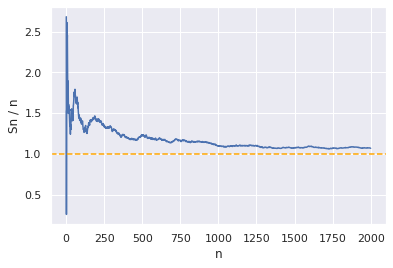
\includegraphics[width = 0.7\linewidth]{"./resources/law_of_large_numbers.png"}
	\caption{Иллюстрация сходимости среднего $ S_n / n $ к матожиданию $ \mu = 1 $ при
	 увеличени $ n $.}
    \label{fig:law_of_large_numbers}
\end{figure}

\begin{figure}[ht]
	\centering
	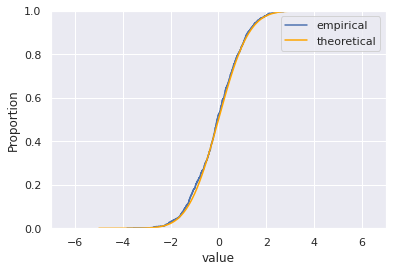
\includegraphics[width = 0.7\linewidth]{"./resources/central_limit_theorem.png"}
	\caption{Эмпирическая функция распределения величины $ \frac{S_n - \mu * n}{\sigma
	 \sqrt{n}} $ при $ n = 1000 $ и теоретическая функция распределения стандартного
	 нормального распределения.}
    \label{fig:central_limit_theorem}
\end{figure}

\anonsubsection{Доверительные интервалы для матожидания и дисперсии}
Построим доверительные интервалы для матожидания и дисперсии, считая их неизвестными.
 Случайная величина
$$
 T = \dfrac{\overline{X} - \mu}{S / \sqrt{n}},
$$
где 
$$
 S^2 = \dfrac{1}{n - 1} \displaystyle\sum_{i = 1}^n(X_i - \overline{X})
$$
--- уже встречавшаяся ранее, несмещенная оценка дисперсии, имеет распределение
 Стьюдента с $ n - 1 $ степенями свободы. Тогда, в силу симметрии распределения,
 получим:
$$
 \mathbb{P} \left( -t_{1 - \frac{\alpha}{2}} \leq T \leq t_{1 -
 \frac{\alpha}{2}} \right) = 1 - \alpha
$$
или же
$$
 \mathbb{P} \left( \overline{X} - t_{1 - \frac{\alpha}{2}} \frac{S}{\sqrt{n}}
 \leq \mu \leq \overline{X} + t_{1 - \frac{\alpha}{2}} \frac{S}{\sqrt{n}} \right)
 = 1 - \alpha,
$$
что непосредственно дает доверительный интервал для матожидания с уровнем доверия
 $ 1 - \alpha $.

Для построения доверительного интервала для дисперсии рассмотрим случайную величину
$$
 H = \dfrac{(n-1)S^2}{\sigma^2},
$$
имеющую распределение хи-квадрат $ \chi_{n-1}^2 $ с $ n - 1 $ степенями свободы.
В данном случае распределение уже не обладает свойством симметрии, поэтому будем
 брать $ \frac{\alpha}{2} $ и $ 1 - \frac{\alpha}{2} $ квантили. В таком случае
 получаем:
$$
\mathbb{P} \left( \chi_{\frac{\alpha}{2}}^2 \leq H \leq \chi_{1 -
 \frac{\alpha}{2}}^2 \right) = 1 - \alpha
$$
или
$$
\mathbb{P} \left( \dfrac{(n - 1) S^2}{\chi_{\frac{\alpha}{2}}^2} < \sigma^2 <
 \dfrac{(n - 1) S^2}{\chi_{1 - \frac{\alpha}{2}}^2} \right) = 1 - \alpha,
$$
откуда немедленно получаем доверительный интервал для дисперсии с уровнем
 доверия $ 1 - \alpha $.
 
Графики доверитльных интервалов для матожидания и дисперсии в зависимости
 от размера выборки, по которой они строятся изображены на Рис.
 \eqref{fig:mean_conf_int} и Рис.\eqref{fig:var_conf_int} соответственно.

\begin{figure}[ht]
	\centering
	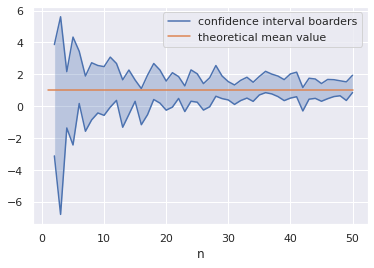
\includegraphics[width = 0.7\linewidth]{"./resources/mean_conf_int.png"}
	\caption{Эволюция доверительного интервала для матожидания $ \mu = 1 $ при
	 увеличении $ n $ с уровнем доверия 95\%.}
    \label{fig:mean_conf_int}
\end{figure}
\begin{figure}[ht]
	\centering
	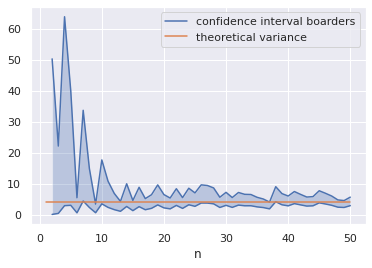
\includegraphics[width = 0.7\linewidth]{"./resources/var_conf_int.png"}
	\caption{Эволюция доверительного интервала для дисперсии $ \sigma^2 = 4 $ при
	 увеличении $ n $ с уровнем доверия 90\%.}
    \label{fig:var_conf_int}
\end{figure}

\anonsubsection{Закон больших чисел и распределение Коши}
Исследуем вопрос справедливости закона больших чисел для последовательностей случайных
 величин Коши. Эмпирически можно сделать вывод, что в отличие от выборок из нормального 
 распределения, сходимость к математическому ожиданию в данном случае отсутствует.
 Это можно объяснить тем, что у распределения Коши вовсе нет математического ожидания,
 а выборочное среднее в выборке из таких случайных величин также будет распределена
 по закону Коши. Иными словами, если $ X_1, \dots, X_n \sim C(a,b) $, то
$$
 \overline{X} = \dfrac{\sum_{i = 1}^n X_i}{n} \sim C(a, b).
$$
Это свойство доказывается с помощью характеристических функций.
\begin{definition}
	Функция $ \phi_X(t) = \Exp e^{itX} $ вещественного переменного $ t $ называется
	 характеристической функцией случайной величины $ X $.
\end{definition}
\begin{statement}
	Характеристическая функция суммы независимых случайных величин равна произведению
	 функций слагаемых.
\end{statement}
\begin{proof}
	Если случайные величины $ X $ и $ Y $ независимы, то, по свойству математческих 
	ожиданий получаем:
	$$
	 \phi_{X + Y}(t) = \Exp e^{it(X+Y)} = \Exp e^{itX} e^{itY} = \phi_X(t) \phi_Y(t).
	$$
\end{proof}
Характеристическая функция однозначно задает распределение, то есть если две случайные
 величины имеют одинаковые характеристические функции, то их распределения совпадают.
 В таком случае, рассмотрим характеристическую функцию выборочного среднего и учтем при
 этом, что для $X_i \sim C(a, b),\ \phi_{X_i} = e^{ait - b|t|} $.
$$
 \psi_{\overline{X}}(t) = \phi_{X_1 + \dots + X_n}\left( \frac{t}{n} \right) = 
  \left( \phi_{X_1(\frac{t}{n})} \right)^n = \left( e^{\frac{ait - b|t|}{n}} \right)^n = 
  \phi_{X_1}(t).
$$
То есть получаем, что $ \overline{X} \sim C(a, b) $. Отсутствие сходимости выборочного
 среднего проиллюстрировано на рисунке \eqref{fig:cauchy_law_of_large_numbers}. На рисунке
 \eqref{fig:sample_mean_cauchy_cdf} проилюстрировано совпадение распределений Коши и
 выборочного среднего для выборки из распределения Коши(так называемого свойства
 устойчивости).
\begin{figure}[ht]
	\centering
	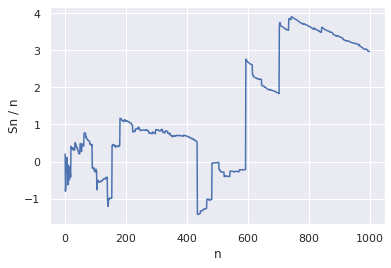
\includegraphics[width = 0.7\linewidth]{"./resources/cauchy_law_of_large_numbers.png"}
	\caption{Поведение среднего значения в выборке из распределений Коши с ростом размера
	 выборки.}
    \label{fig:cauchy_law_of_large_numbers}
\end{figure}

\begin{figure}[ht]
	\centering
	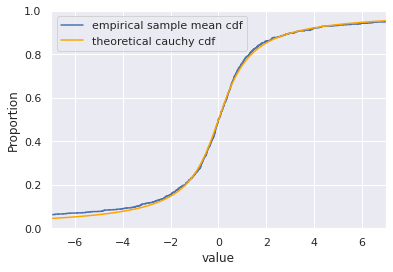
\includegraphics[width = 0.7\linewidth]{"./resources/sample_mean_cauchy_cdf.png"}
	\caption{Иллюстрация устойчивости распределения Коши: $ \overline{X} \sim C(a, b) $. 
	 $ a = 0,\ b = 1 $}
    \label{fig:sample_mean_cauchy_cdf}
\end{figure}